\subsection{Results}
To keep the presentation clear, tables and plots show mean scores without standard-deviation annotations.
\begin{center}
\begin{minipage}{\linewidth}
\centering
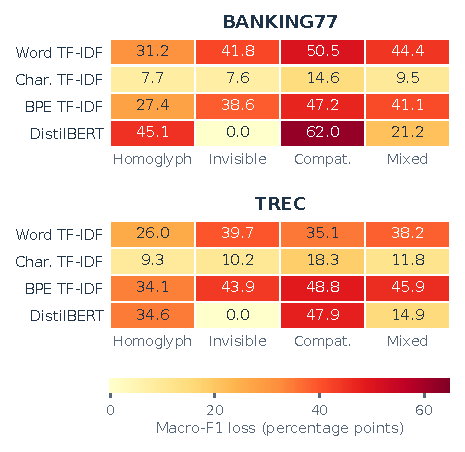
\includegraphics[width=\linewidth]{attack_family_comparison.pdf}
\captionof{figure}{Macro-F1 loss at 20\% strength, without defenses (larger is worse). Mixed is not always the hardest attack: on BANKING77, DistilBERT loses 62.0 points to compatibility changes, 21.2 to mixed attacks and none to invisible controls. Composition is omitted because it changes no inputs.}
\label{fig:attack-family-comparison}
\end{minipage}
\end{center}

\minisection{Clean accuracy does not settle the robustness comparison}
Character TF--IDF has the strongest clean BANKING77 score, while DistilBERT leads on TREC. At the main 20\% strength setting, character features retain the highest average Macro-F1 on both datasets (Table~\ref{tab:performance}). Their attack-success rates are also the lowest: fewer initially correct predictions are overturned.

\begin{table*}[!tbp]
\centering\small
\caption{Clean and attacked test performance. Attacked F1, loss and ASR average the four effective families at 20\%.}
\begin{tabular}{@{}lrrrrr@{}}
\toprule
\tabhead Model & Clean acc. & Clean F1 & Attacked F1 & F1 loss & ASR \\
\midrule
\multicolumn{6}{l}{\textbf{BANKING77}} \\
Word TF-IDF & 0.885 & 0.886 & 0.466 & 0.420 & 49.0\% \\
Character TF-IDF & 0.906 & 0.906 & 0.807 & 0.099 & 12.5\% \\
BPE TF-IDF & 0.882 & 0.882 & 0.496 & 0.386 & 45.3\% \\
DistilBERT & 0.832 & 0.819 & 0.498 & 0.321 & 40.8\% \\
\addlinespace[5pt]
\multicolumn{6}{l}{\textbf{TREC}} \\
Word TF-IDF & 0.888 & 0.885 & 0.537 & 0.347 & 38.6\% \\
Character TF-IDF & 0.888 & 0.883 & 0.759 & 0.124 & 17.9\% \\
BPE TF-IDF & 0.890 & 0.879 & 0.447 & 0.432 & 45.4\% \\
DistilBERT & 0.967 & 0.944 & 0.701 & 0.243 & 27.4\% \\
\bottomrule
\end{tabular}

\label{tab:performance}
\end{table*}

\begin{figure}[H]
  \centering
  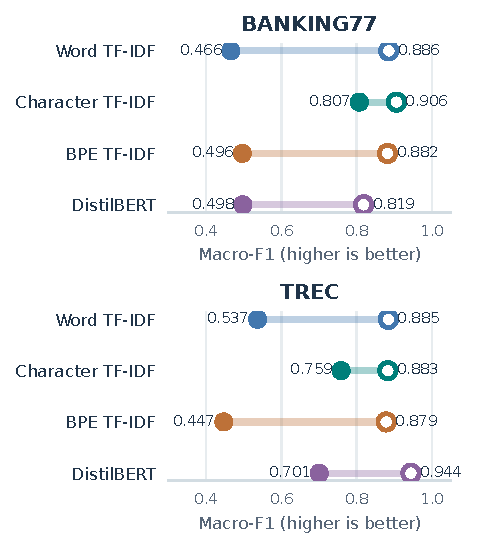
\includegraphics[width=\linewidth]{performance_overview.pdf}
  \caption{The main result at a glance. Filled points show averaged Macro-F1 at 20\% perturbation, hollow points show clean performance.}
  \label{fig:overview}
  \vspace{1 mm}
\end{figure}



\minisection{Performance across the full attack-strength range}
Figure~\ref{fig:robustness} follows all measured strengths. Mean Macro-F1 decreases and attack success rises as more eligible positions are changed. Character features lead on BANKING77 throughout. On TREC, DistilBERT leads at 5\% (0.865 versus 0.853); character features lead from 10\% to 40\%, but DistilBERT leads again at 75\% (0.411 versus 0.337). All four models are evaluated through 75\%.

\begin{figure}[H]
\centering
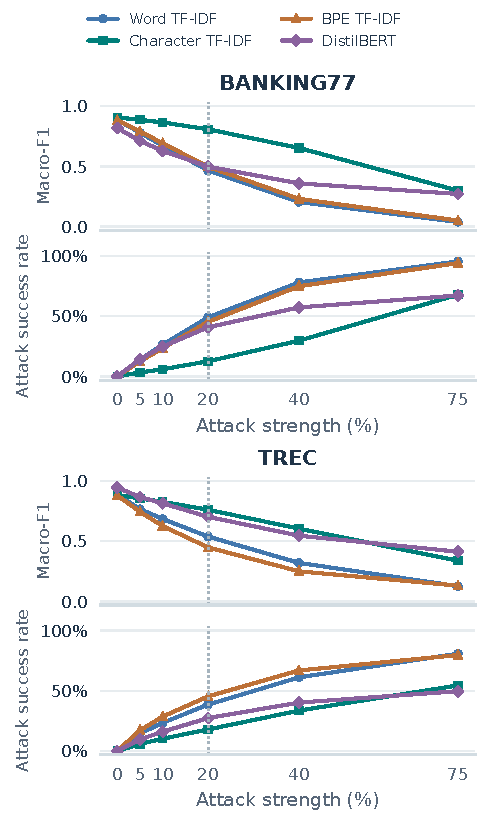
\includegraphics[width=\linewidth]{attack_strength_overview.pdf}
\caption{Macro-F1 (higher is better) and attack success rate (lower is better), averaged equally across four effective families. Zero denotes clean text; the dotted line marks 20\%.}
\label{fig:robustness}
\end{figure}

\minisection{What remains at 40\% and 75\%?}
The stronger attacks reveal substantial losses even for the most robust representation (Figure~\ref{fig:strong-attacks}).
On BANKING77, character Macro-F1 falls from 0.653 at 40\% to 0.299 at 75\%, while word and BPE features reach 0.039 and 0.051. DistilBERT reaches 0.271. At 75\%, attacks overturn 67.8\% of the predictions that the character model got right when clean.

On TREC, character Macro-F1 falls from 0.603 at 40\% to 0.337 at 75\%, while word and BPE features reach 0.126 and 0.130. DistilBERT reaches 0.411. At 75\%, attacks overturn 54.4\% of the predictions that the character model got right when clean.


\begin{figure}[H]
\centering
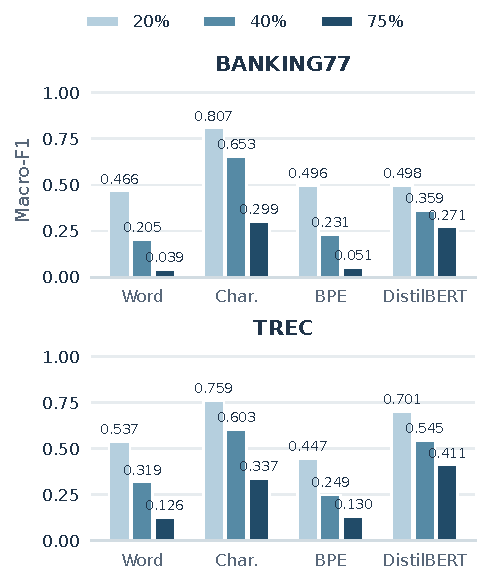
\includegraphics[width=\linewidth]{strong_attack_comparison.pdf}
\caption{Mean Macro-F1 at 20\%, 40\% and 75\%, using the same four-family average.}
\label{fig:strong-attacks}
\end{figure}

\minisection{The attack family changes the trajectory}
The family breakdown in Figure~\ref{fig:families} explains why the mean alone is incomplete. DistilBERT stays at its clean score under the tested invisible controls through 75\%, while its BANKING77 Macro-F1 heavily suffers under compatibility substitutions . Its preprocessing discards the tested invisible characters. Character features also degrade: compatibility substitutions give them the lowest 75\% score on both datasets. Mixed attacks sample applicable transformations and as such will not necessarily perform like the worst single family.

\begin{figure}[H]
\centering
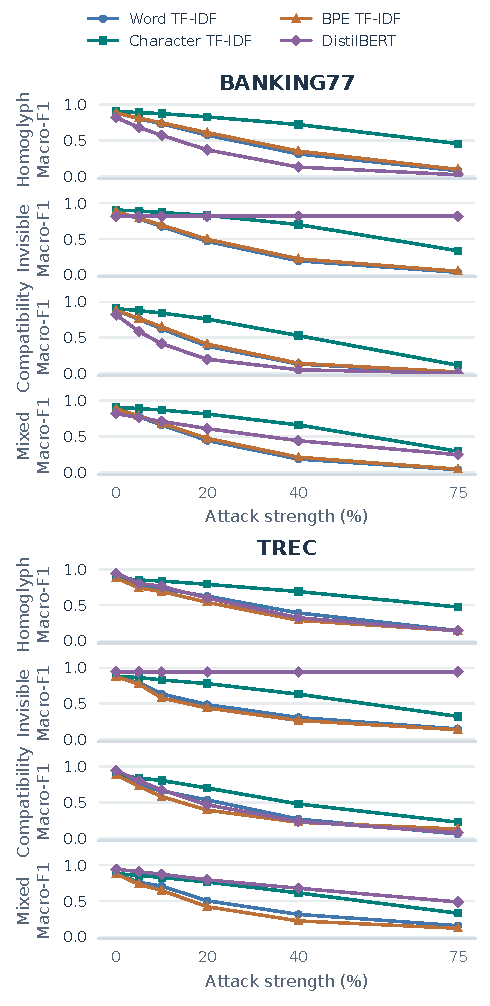
\includegraphics[width=\linewidth]{attack_strength_by_family.pdf}
\caption{Macro-F1 by attack family and dataset across all available strengths. Each curve begins at its clean score. Composition is omitted because it changes no test inputs. All four models cover the full range through 75\%.}
\label{fig:families}
\end{figure}

\Needspace{0.7\textheight}
\minisection{How much of the lost score is recovered?}

\begin{figure}[H]
\centering
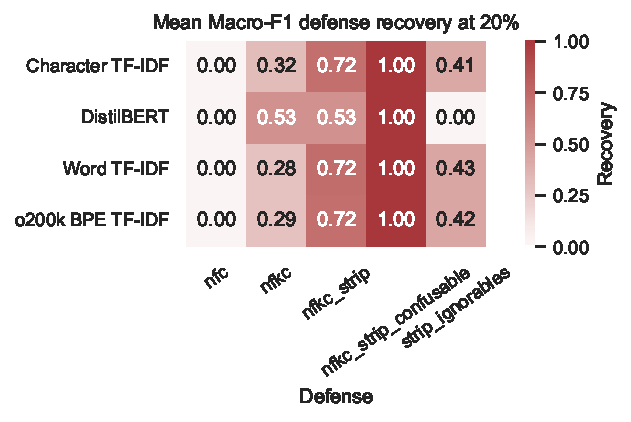
\includegraphics[width=\linewidth]{defense_recovery.pdf}
\caption{Macro-F1 before and after repair, averaged across the four effective families at 20\%. Full repair nearly reaches the clean baseline; its map covers the restricted attack whitelist.}
\label{fig:defense}
\end{figure}


\begin{table*}[!tbp]
\centering\small
\caption{Mean defense recovery at 20\% strength, shown as \(100R\): 72.31 means 72.31\% of the lost score recovered on the equal-family average. Each classical row averages four defined family ratios. DistilBERT averages three, excluding invisible attacks because their raw score loss is zero. Rounded 100.00 values need not imply exact recovery.}
\begin{tabular}{@{}lrrrrr@{}}
\toprule
\tabhead Model & NFC & NFKC & Removal & NFKC + removal & Full repair \\
\midrule
\multicolumn{6}{l}{\textbf{BANKING77}} \\
Word TF-IDF & 0.00 & 28.66 & 42.96 & 72.31 & 99.98 \\
Character TF-IDF & 0.00 & 31.00 & 42.67 & 72.29 & 100.00 \\
BPE TF-IDF & 0.00 & 29.18 & 43.13 & 72.43 & 99.98 \\
DistilBERT & 0.00 & 54.42 & 0.00 & 54.42 & 99.99 \\
\addlinespace[5pt]
\multicolumn{6}{l}{\textbf{TREC}} \\
Word TF-IDF & 0.00 & 28.17 & 42.67 & 72.06 & 100.00 \\
Character TF-IDF & 0.00 & 32.28 & 40.21 & 70.86 & 100.00 \\
BPE TF-IDF & 0.00 & 28.27 & 41.63 & 70.98 & 99.99 \\
DistilBERT & 0.00 & 51.97 & 0.00 & 51.97 & 100.00 \\
\bottomrule
\end{tabular}

\label{tab:defense-recovery}
\end{table*}

Combining NFKC and control removal improves classical recovery because they repair different families. DistilBERT already discards the tested controls, so removal adds nothing. Its combined recovery is 54.42\% on BANKING77 and 51.97\% on TREC over three attack families (not the homoglyph).

\minisection{A worked recovery calculation}
\label{sec:recovery-example}
For BANKING77 word TF--IDF under the 20\% mixed attack, clean Macro-F1 is 0.885686, raw attacked Macro-F1 is 0.441687, and NFKC plus removal raises it to 0.837951. Applying Equation~\ref{eq:recovery} gives:
\begin{equation*}
R_{\mathrm{mixed}}=\frac{0.837951-0.441687}{0.885686-0.441687}\approx 0.892.
\end{equation*}

The defense recovers 89.2\% of this loss. Its four-family mean is 72.31\%: compatibility and invisible attacks are fully repaired, while homoglyphs are not. Calculating \(R\) from cross-family average scores would weight families by their initial loss; the table instead averages their recovery ratios equally.
 Near-complete recovery is measured on this restricted attack set.